\definecolor{verbgrey}{gray}{0.85}

\section{Implementation}
This project was developed over 8 sprints of between 7-10 days each with the first one started on the 26th of December, 2022 and the last one stared on March 19, 2023. What follows is a detailed summary of the work done during those sprints divided into three subsections:
\begin{itemize}
    \item Plan - Highlights what user stories were chosen to be implemented during the sprint and how long that sprint was.
    \item Implementation - How the features were implemented, any design decisions and any issues
    \item Summary - Have all user stories been completed? What went wrong? Anything learned and moved to next sprint
\end{itemize}

\subsection{Sprint 1 - Start 26th December}

\subsubsection{Plan}
This was the first sprint undertaken for the project and so the focus was to test everything out and ensure that the process was right for the student. The initial MVP feature set was chosen for development and two user stories were planned for. Those being user stories 3 and 11 with a total workload estimate of 6 over a 7 day sprint.
The main goal for this sprint was to create a labelled scatterplot graph with some pre-set test data.

\subsubsection{Implementation}
Prototype 2 was chosen to be extended into the application being developed. It was copied into the development branch and work started on implementing the user stories mentioned. A 3D Cube with axis lines was created as the chart and an origin position was set from which data points would be rendered. This was not as difficult as expected as the model matrix used could be copied and modified by each data point to ensure that they were always at a correct position relative to the cube and axis lines.

The next step was to label the axis lines (also relative to the chart using it's model matrix). This caused some difficulty as test labels would not align properly even if they were supposed to based on their coordinates. This was particularly troublesome with perspective lines that had a considerable z change in position. This was found to be a result of inaccurate placement by the browser (browsers favors flexibility over screen sizes instead of rigid pixel-perfect placement) and not fully correct world to screen coordinate calculation. Instead, it was decided that text should be rendered within the WebGL scene to ensure accuracy- To that end, a bitmap font technique was adopted.

\begin{figure}[h]
    \centering
    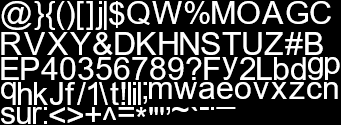
\includegraphics[width=0.5\columnwidth]{author-files/figures/glyphset.png}
    \caption{Arial font bitmap glyph image}
    \label{fig:arial}
\end{figure}

This is where a texture atlas with pre-rendered glyphs is downloaded and used to apply individual glyphs to flat surfaces (usually two triangles of geometry). This technique was mainly adopted due to it's simpler implementation and higher performance over the main alternative of using a geometric approach for rendering text (Where geometry is used to shape each glyph, which uses much more triangles). This alternative is highly inefficient as geometry is computationally expensive to render. Although it should be noted that bitmap font's do also carry their own limitations, mainly it is difficult to have large character sets as each character set would need to be saved into an image and downloaded, which if changing font sizes is required further requires that different sized copies of the character sets are available to avoid blurriness and pixelation at large sizes.
For this project though, those were considered to be tolerable limitations. Blurriness could be avoided by keeping glyphs the same size and the limited glyph set wouldn't matter as much with only one supported application language.
With bitmap fonts decided upon, the student started work on adapting the application to support rendering text in this way. This required a couple of key changes and additions within the renderer part of the application:
\begin{itemize}
    \item It should be possible to apply textures to models- This was done by adapting the Model class to store and apply texture data on render
    \item Textures had to rendered and stored- This was done by expanding the Loader class to allow .png images to be loaded
    \item There had to be some way to abstract which letter was rendered, manually slicing the bitmap texture to get each glyph would quickly become too tedious and time consuming for anything beyond a few glyphs- A State-Machine based Font Class was created that generated font texture data for an input letter that could be fed into a Model Object.
\end{itemize}

Have some class diagram here

\subsubsection{Summary}
The new technique for rendering text ended up fixing the accuracy issues caused by the previous label system and all user stories managed to be completed as expected and the application was pushed to production on january 1st, 2023. This was a slow start but the student expected that more user stories would be able to be tackled as they progressed with the project.

\subsection{Sprint 2 - Start 4th January}
\subsubsection{Plan}
This was the second sprint and the plan was to start adding user controls to allow a user to modify what was being rendered. This included not only the ability to upload custom data but also rotate the resultant graph. The MVP feature set was again the developed feature set from which 4 user stories were selected, with a total work load estimate of 16 over a longer 11 day sprint. This was originally a 7 day sprint but an extension was deemed necessary to have an atomic conclusion to the sprint. In total, 16 Units of work were completed for an average of 8 per week.

\subsubsection{Implementation}
Loader was once again expanded to handle .csv loading which was done using jquery-csv, which sped up development considerably and covered a lot of edge cases in possible file uploads. For user controls, the use of modern UI frameworks was considered but at this moment in time- there wasn't much UI requirement for the application. Instead, as per PXP, the student focused on hitting user stories as fast as possible. Thus, an observer like structure was implemented using Event listeners connected to overlaid HTML Elements on the page (In a similar way to how the old label system worked, See Sprint 1) which ran functions that modified the state of the application. With this design, 6 buttons were made to rotate each axis of the chart individually. Another button was added to upload a file that was handed to Loader.

During this time, when implementing rotation- which consisted of applying a rotating model matrix component to the entire scene. An expected issue cropped up of having to rotate glyphs to always face the camera even when the scene rotates. This consisted a task that needed a billboarding shader to be written that was used when text is rendered in the application.

\subsubsection{Summary}
This was almost a double sprint. This was mainly due to lower work hours done by the student during the winter vacation. Nevertheless, All user stories were completed and the application was pushed to production on January 29th. This delay was due to the previously mentioned lower hours and semester start travel. At this point, a technically functional plotter was created, though still very limited in functionality.

\subsection{Sprint 3 - Start 29th January}
\subsection{Plan}
This was the third sprint and first sprint undertaken during semester 2. The plan was to tackle some of the biggest requirements from the MVP feature set- in turn making the application more capable. A total of 6 User stories were selected with one of them, story 6 alone being ranked at a workload of 10. In total, the sprint consisted of 25 work load points over a period of 12 days. This was the biggest sprint undertaken to date but the student was confident in rising up to the challenge. Some of the sprints assigned to this sprint were tackled in previous sprints but were not developed to a suitable standard of quality to qualify to be committed.

\subsubsection{Implementation}

One of the user stories was to implement the ability to change what slice the graph showed / what the axis values are. This is the beginning of adding dynamic navigation to the data that was mentioned in the design. During this sprint, this idea of navigation was distilled down into 2 essential parts. With that being:
\begin{itemize}
    \item Moving the chart "slice" in each axis. An example would be if a 1-10 on each axis chart is moved +1 in the y direction the chart x, z axis would still show 1-10 but the y axis will now show 2-11.
    \item Zooming. This can be considered as increasing the size of the slice shown by a chart. If a 1-10 on each axis slice chart is scaled to a factor of 2x it would now show 1-20 on each axis.
\end{itemize}

Before any of these could be implemented though, glyph rendering had to be reworked to allow values consisting of more than one digit to be shown at each labelled line of the chart. This was a relatively straight-forward addition where instead of a single glyph being rendered at each line, an array of glyphs was rendered instead. With each digit of a number being a single glyph in order stored in the array.

Moving the chart was then started to be implemented. This was done by adding new movement buttons (2 for each axis that either moved the axis ahead by 1 by back by 1) then using event listeners getting the modification value and applying it calculate the range of axis vales that needed to be rendered (This was at most 10 values). These values were then applied in order for each labelled line on the chart. This was a relatively straight forward addition.
\begin{figure}[h]
    \centering
    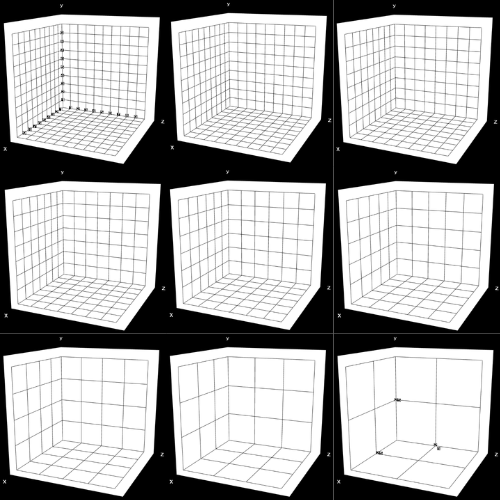
\includegraphics[width=1\columnwidth]{author-files/figures/oldzooms.png}
    \caption{Zooming effect formed by Axis Lines (Zooming Out)}
    \label{fig:oldzoom}
\end{figure}

Zooming was one of the most challenging features of this project to implement. The implementation at this time attempted to create a visually pleasing effect where axis lines would move out to give the illusion that the camera was moving closer without actually changing camera position nor size of the viewing graph cube. This was an easy enough effect to achieve and one that could correctly sync up with the position of data cubes too.

\begin{code}
    glmath.mat4.translate(
    Axismodel, // Model Matrix in var
    Axismodel, // Resultant Matrix var
        [0.5, 0, (i / (10 * zoom))]);
\end{code}

For cubes the effect could be applied simply as:
\begin{code}
    glmath.mat4.translate(
    point_model, // Model Matrix in var
    point_model, // Resultant Matrix var
        [x * zoom, y * zoom, z * zoom]);
\end{code}

The problem then, was correctly labelling axis lines at every possible state of zoom level. In other words, Even though positionally the cubes and axis lines were correctly placed at all zoom levels- figuring out what the exact values of each line were was very challenging., this was further exacerbated by the ability "move" the graphed slice to show different values. After extensive tinkering, labels were turned off when the application was in an uncertain state- As a temporary solution, a hardcoded zoom modifier was set for maximum and minimum zoom values (These were the only levels at which the zoom mod values could be confirmed as correct) allowing accurate labels to be shown at those two levels.
With this, the application could now zoom up to a maximum of 5x showing values from 0 to 50 and a minimum of 1 to 10 at 1x. In between those two maximum and minimum levels (including those levels) there were 10 pre-set zoom values that could be scrolled through.

\subsubsection{Summary}
This was one of the most important sprints undertaken in terms of extending chart capabilities. All mentioned user stories were completed and the application was pushed to production on February 9th. At the end of this sprint the application was starting to become ready for user testing and could technically handle most data- Further information on user testing is mentioned in section X.

\subsection{Sprint 4 - Start February 10th}
\subsubsection{Plan}
This was the fourth sprint. The main driving factor during this sprint was to prepare the application for user testers. To that end, 4 user stories were selected with a total workload of 10. These all focused on critical UI accessibility problems that would likely otherwise dominate user feedback. The sprint was planned to run for 6 days.

\subsubsection{Implementation}
This was a relatively straight forward sprint. No major systems or additions were added and most work used the UI Observer pattern using Event listeners as previously defined for UI needs. Although it was starting to become noticeable that adding more controls was starting to affect code quality and maintainability. A refactoring task was added to the backlog to look at opportunities to restructure the app.

\subsubsection{Summary}
The sprint was completed in record time. All user stories were implemented and the app was pushed to production on Feb 12, two days after the sprint started. The remaining time was instead reallocated to plan for user testing. At this point, the application could not only render most data but had reasonable ability to display that data correctly and provide basic user controls to that end. It would now be important to get user feedback to drive the application forward beyond it's most basic state.

\subsection{Sprint 5 - Start February 19th}
\subsubsection{Plan}
This was the fifth sprint. User testing 1 has already started at this point in time and the student was waiting results to finish come in before analysis could start.
In this relative downtime. A 7 day sprint was planned with 2 user stories for a workload of 9 points. These were task based stories that arose during development in previous sprints, and the student thought they would be important additions to have.

\subsubsection{Implementation}
The first story was to display names for each axis taken from the first row of the dataset. This was pretty straight forward thanks to the Font + Model Abstraction and was promptly implemented.

The next user story though was to look at new ways to structure the app to increase maintainability. The main areas of opportunity thus found were as follow:
\begin{itemize}
    \item Restructure application to be fully Object-Oriented - At the moment the application is a script that extensively uses Objects (From classes such as Model and Loader) to implement the chart in a high level as a result of the abstractions provided by those objects. This is fine and probably the best design for a single chart to be rendered but there may be potential for further abstraction to allow multiple charts per page that can interact with each other.
    \item Find a way to better manage UI state. This is currently not a problem with the relatively simple user controls but may become cumbersome when more controls are added and if some controls might start being dependant on other controls.
    \item Find an overarching architecture to manage UI and Rendering code.At the moment user controls are highly coupled to rendering which is not ideal. It would be best to decouple them in some way to make adding more UI components easier.
\end{itemize}

Each of these points were researched in turn and prototyped with in turn. Although time was a very limited factor as the student considered it important to provide value to the user first and foremost. Which meant refactoring would likely not be able to continue beyond this 7 day sprint as requirements extracted from user testing would then be higher prioritized. First, some attempts were made to restructure the render loop into an object but it was more work than expected to port everything correctly so it was abandoned.

As for state management, there were a number of techniques and pre-made solutions for managing state. React + React Context though, has been found to be a great fit for the project. React is a UI library for creating user interfaces through components and now has support for state management by sharing states between these components. Parcel also has great support for react so integration would not have been too problematic. Unfortunately, the unique circumstances of this project made the student reject integrating react into the tool stack at the current time for the following key reasons:
\begin{itemize}
    \item Performance cost. Although most likely negligible, there is still none the less a performance cost in using an abstraction such as react. This is particularly important as the application already was performance heavy due to 3D rendering.
    \item Lack of time and experience. In a perfect world the library could be easily implemented with no downtime and no future issues. Unfortunately, the reality is that adding react would have heavily changed the tech stack that could cause unknown problems. This is further exemplified by the student not having any considerable experience in using react meaning any issues that did pop-up would be much more difficult to solve. There was also no time to have a prototyping phase to mitigate these concerns as there was with the current stack at the start of this project.
    \item Minimal Value added. As previously mentioned the current system worked as needed and did not need any changes to provide further functionality to the user. As such, it would have been hard to justify work done of porting the application to react over only future concerns. PXP prioritizes doing the simplest design and not worrying about future requirements as those tend to change constantly.
\end{itemize}

The final point, to find an overarching architecture, the student found that the application fit very well into the MVC pattern. As such, the student starting working on implementing the pattern- which went smoothly as the application had already been unknowingly made to partially fit the pattern by the student.
The application was structured as follows:
\begin{itemize}
    \item View - Static Written HTML index.html
    \item Model - The application render loop rendering chart. The chart rendered is a result of multiple control variables which make up the model.
    \item Controller - This was the new class created. All event listeners and control functions were moved to be managed by this class.
\end{itemize}
Have chart showing all this here TODO

\subsubsection{Summary}
This was an important sprint that worked to refactor the application to be easier to work with, especially when adding new UI elements.
The 2 user stories were thus completed and the application pushed to production as Version 2 on March 4th.
It was completed just in time as user testing has come to a close and analysis begun.

\subsection{Sprint 6 - Start March 05}
\subsubsection{Plan}
This was the 6th Sprint, and the first sprint starting work on the second version of the project. Two new FeatureSets were now available for user stories to be selected from. One composed from user testing analysis as further described in section X and A further improvements feature set created in a similar fashion as the first MVP feature set (By the student through the research phase). For this Sprint, 7 Stories were selected from both feature sets with a priority for Must. In terms of workload, a wide range were selected for a total workload of 27 Points over a 5 day sprint period.

\subsubsection{Implementation}
The first important story done was reworking how zooming worked. User testers asked for a zoom that showed labels for each level which was found to be difficult to calibrate with the zooming visual effect as mentioned in Sprint 3. So instead, the zoom was reworked to always show 10 axis lines and only change position of data points and labels on zoom- This was generally straight forward and created a robust zoom that hit the criteria, even if it didn't look as visually impressive.

The next addition was to modify the renderer to allow picking / highlighting data points. To achieve this, two main techniques were identified by the student.
\begin{itemize}
    \item Raycasting - This works by taking the screen coordinates clicked on by the user and projecting them into the 3D scene. From this scene position a ray is then shot and a check done to get any intersections with objects.
    \item Colour Picking - This is a technique where Object ID is encoded into the colour of an object. When a user then clicks on an object, it is possible to get what object was clicked on by picking the colour at the click position (pixel clicked on) and matching it to an object in the scene.
\end{itemize}

After analysis of the two, Colour picking was chosen over ray tracing for the following key points:
\begin{itemize}
    \item More Complex implementation with raycasting.
    \item Raycasting is highly CPU dependant, Lots of Math- which isn't good with JavaScript.
    \item Something else
\end{itemize}

To implement colour picking then, the student extended the renderer to render data points twice- The first render would render to a texture in a different buffer, this first render would also encode an ID for every Model rendered into 3 rgb Channels giving a unique colour for every model drawn (up to around 16 million). After that, render is called again but to the screen buffer instead. This means that the user only see's the the second render (Which can freely use colour) instead of the first one.
*Have image comparison here*

glGetPixel would then poll what colour pixel the user's mouse is hovering over. During the second render phase as each model is rendered, it's id is checked to see if it matches the selected id extracted from the colour of the hovered over pixel. If it does, the model is highlighted and it's data saved to be displayed.

\subsubsection{Summary}
All User stories were completed as expected and the application pushed to production on March 11. With this sprint almost all Must stories from both Feature sets making this a very productive sprint and one that set the project on good track to be completed by the end of the month.

\subsection{Sprint 7 - Start March 12}
\subsubsection{Plan}
This was the 7th Sprint. The highest priority user stories were once again selected from both feature sets. This included the last 2 Must stories and 2 Should stories. In total, the workload was 21 over a 5 day period. The main focus of this sprint was to expand the application to support one more dimension and create a new suite of user controls to view and assign data to chart axies.

\subsubsection{Implementation}
To add a new dimension, the student had to start looking at different ways to represent dimensions. The main options identified were Alpha/Transparency, Single Channel / Saturation component, Full Colour component and Shape component.
Of those, Shape was dropped due to limited range (Have to have a different model to represent each possible values). Alpha was also dropped due to difficulties in how the browser handles Alpha. Finally, Saturation was chosen over colour as having all 3 channels might be confusing for users to extract values.

During the following implementation- the first problem encountered was how to plot an infinite range of values between two Saturation values on a single channel. For this problem the student identified the use of a squashing function that formed an asymptote at the limits. By then also allowing the user to change those limits, any data can be effectively plotted with saturation.

\begin{figure}[h]
    \centering
    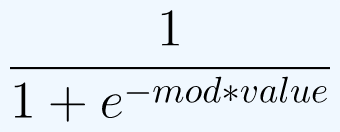
\includegraphics[width=0.5\columnwidth]{author-files/figures/squashFunc.PNG}
    \caption{Squashing Function, where mod is based changed by the user while value is the value of the data point plotted}
    \label{fig:function}
\end{figure}

Once the mathematical basis was solved, the implementation was relatively straight forward.
The next main addition worked on was to create a new section of user controls. To that end, a tabular design was adopted for aspects of the application that demanded large screen real estate and focus from the user. This consisted of three total tab sections as follows:
\begin{itemize}
    \item Graph View - This is what has been shown so far, the rendered graph.
    \item Data Management - This will be a new tab. Here, the data uploaded is displayed in a table fashion with data point IDs for cross reference with the graph. Additionally, a set of selectors were created on the page that allowed the user to select which column from the table would apply to which axis to be graphed (or to saturation).
    \item Help tab - This is a FAQ based help section, Answers to common (or expected to be) questions.
\end{itemize}

This was also relatively straight forward to implement, although with the data management tab- the UI system was pushed to it's limit in terms of state management. The student had to design the UI in such a way as to minimize UI elements depending on each other for state. Although there still are nevertheless some less than ideal control implementations. *Have example here*. Any considerable future UI work will preferably need to bring on some helping tool to minimize development time and complexity.

\subsubsection{Summary}
All user stories were completed as expected and the application was pushed to production on March 18th. The usability of the application took a considerable upgrade this sprint- with the application itself being almost fully completing both feature sets.

\subsection{Sprint 9 - Start March 19}
\subsubsection{Plan}
This was the 9th sprint and expected to be the last sprint before user testing 2 could start. Only 2 user stories were selected for development with a total workload of 3 points over a 5 days span.Most of the time this sprint was dedicated to preparing for user testing over development. Nevertheless this was still an important sprint that covered some of the last few to be implemented Should stories.

\subsubsection{Implementation}
Implementation went as expected. The stories mainly needed some minor UI additions.

\subsubsection{Summary}
All stories were completed and the application was pushed to production on March 29th. With this sprint, the application was ready to be user tested again.

